\section{A topos with countable reals}
\label{sec:topos-with-countable}

Given a Miller sequence~$\mil$, as in~\cref{sec:non-diag-sequ}, let~$\MM{\mil} \defeq \invim{\srep}(\mil)$ be the set of all oracles representing~$\mil$ where $\srep$ is the representing map from \cref{sec:oracle-comp-maps}. Define $\TT{\mil} \defeq \PRT{\KK,\MM{\mil}}$ to be the parameterized realizability topos constructed from the ppca $\KK$ with oracles $\MM{\mil}$, see \cref{ex:oracle-ppca}.

\subsection{Countability of the reals}
\label{sec:countability-reals}
%
Let us immediately address countability of the Dedekind reals in~$\TT{\mil}$. 
We first reduce the problem to countability of the closed interval.

\begin{lemmaC}
  \label{lem:R-contable-iff-I-countable}%
  The real numbers are countable if, and only if, the closed unit interval is countable.
\end{lemmaC}

\begin{proof}
  If $\RR$ is countable then $[0,1]$ is countable because there is a retraction $\RR \to [0,1]$, for instance
  $x \mapsto \max(0, \min(1, x))$.
  %
  Conversely, given $e : \NN \to [0,1]$ is a surjection, we claim that $e' : \NN \to \RR$, defined by
  $e'(\pair{m, n}) \defeq m \cdot (2 \cdot e(n) - 1)$, is a surjection also. For any $x \in \RR$ there is $m \in \NN$ such that
  $-m < x < m$, and there is $n \in \NN$ such that $e(n) = \frac{x + m}{2 m}$, hence $e'(\pair{m, n}) = x$.
  %
  % computation of e'(<m, n>):
  % e'(<m, n>) = m (2 e(n) - 1)
  %           = m (2 ((x + m)/(2m)) - 1)
  %           = m ((x + m)/m - 1)
  %           = m (x/m)
  %           = x.
\end{proof}

Next, we obtain custom descriptions of the assemblies of natural numbers and the closed unit interval.

\begin{lemma}
  \label{lem:nno-assembly}%
  In the topos $\TT{\mil}$ the natural numbers object is isomorphic to the assembly $\objN$ with carrier
  $\carrier{\objN} \defeq \NN$ and the existence predicate
  %
  $\Ex{\objN}(n) \defeq \set{n}$.
\end{lemma}

\begin{proof}
  In \cref{sec:natur-numb-integ} we saw that the natural numbers object is the assembly with carrier
  $\NN$ and existence predicate $n \mapsto \set{\numeral{n}}$. The assembly from the statement is isomorphic
  to it because we may convert between $\numeral{n}$ and $n$ using the combinators~$\combNum$ and~$\combCur$ from \cref{ex:numers-vs-numerals}.
\end{proof}

Henceforth we use~$\objN$ from \cref{lem:nno-assembly} as the standard natural numbers object. The practical consequence is that we may eschew Curry numerals and instead use numbers directly.

\begin{lemma}
  \label{lem:interval-assembly}%
  In the topos $\TT{\mil}$ the closed unit interval is isomorphic to the assembly $\objI$ with carrier
  $\carrier{\objI} \defeq [0,1] \cap \carrier{\RRd}$ and the existence predicate
  %
  $\Ex{\objI}(x) \defeq \set{m \in \KK \such \mil(m) = x}$.
\end{lemma}

\begin{proof}
  The sub-assembly $\set{x \in \RRd \such 0 \leq x \land x \leq 1}$ has $[0,1] \cap \carrier{\RRd}$ as its carrier set. Its existence predicate is the tripos predicate
  %
  $[x \of \RRd \such 0 \leq x \land x \leq 1]$,
  %
  which is $\neg\neg$-stable, and therefore equivalent to $\Ex{\RRd}(x)$ restricted to~$\carrier{\objI}$.
  %
  Thus, it suffices to show that the tripos logic validates
  %
  \begin{equation}
    \label{eq:objI-ER-to-EI}
    %
    x \of \carrier{\objI} \such \Ex{\RRd}(x) \to \Ex{\objI}(x).
  \end{equation}
  %
  and
  %
  \begin{equation}
    \label{eq:objI-EI-to-ER}
    x \of \carrier{\objI} \such \Ex{\objI}(x) \to \Ex{\RRd}(x).
  \end{equation}
  %
  By \cref{cor:dedekind-characterization}, $\R{r} \in \Ex{\RRd}(x)$ is equivalent to
  %
  \begin{equation}
    \label{eq:objI-rz-x}
    \all{\alpha \in \MM{\mil}}
    \all{k \in \NN}
    |x - \rat{\pr[\alpha]{\R{r}}(k)}| < 2^{-k},
  \end{equation}
  %
  where we used $\objN$ from \cref{lem:nno-assembly}.
  %
  Condition \eqref{eq:objI-rz-x} states that~$\R{r}$ is a $\mil$-index for~$x$ in the sense of \cref{def:sequence-computable}, therefore $\mil(\R{r}) = x$ and we may realize \eqref{eq:objI-ER-to-EI} with $\ucode{\abstr{r} r}$.

  It remains to realize \eqref{eq:objI-EI-to-ER}.
  %
  In \cref{sec:oracle-comp-maps} we obtained $\R{v} \in \NN$ such that, if~$\alpha$ codes $\mil$ then
  $\pr[\alpha]{\R{v}}(m)$ represents $\mil(m)$, for all $m \in \NN$.
  Clearly, $\R{v}$ realizes \eqref{eq:objI-EI-to-ER}.
\end{proof}

\begin{theorem}
  \label{thm:countable-reals}
  In the topos $\TT{\mil}$ there is an epimorphism from natural numbers to Dedekind reals.
\end{theorem}

\begin{proof}
  By \cref{lem:R-contable-iff-I-countable,lem:interval-assembly} it suffices to show that the Miller sequence $\mil : \objN \to \objI$, which is realized by $\ucode{\abstr{m} m}$, is an epimorphism. This is so because
    %
  \begin{equation*}
    \all{x \in \objI} \some{m \in \objN} \mil(m) = x
  \end{equation*}
  %
  is trivially realized by $\ucode{\abstr{m}{m}}$ as well.
  %
  % Verification: the topos statement computes to the following tripos predicate:
  % [ ∀ x ∈ I . ∃ m ∈ N . μ(m) = x ] =
  % [ ∀ x : |I| . E_I(x) → ∃ m ∈ ℕ . E_I(μ(m)) ∩ E_I(x) ] =
  % [ ∀ x : |I| . E_I(x) → ∃ m ∈ ℕ . E_I(μ(m)) ∩ E_I(x) ]
  %
  % Given any x ∈ |I| and r ∈ E_I(x), there is m ∈ ℕ such that r = i(m) and μ(m) = x.
  % So we get E_I(μ(m)) ∩ E_I(x) = E_I(x) and (α | (⟨m⟩ m) r) = (α | r), as required.
\end{proof}

\subsection{What else is countable?}
\label{sec:what-else-countable}
%
Given that \cref{thm:fixed-point-R-uncountable,thm:countable-reals,thm:cauchy-uncountable} sandwich the countable Dedekind reals between uncountable Cauchy reals and uncountable MacNeille reals, it is natural to wonder about which classically uncountable spaces are countable in~$\TT{\mil}$.

Products, sums and images of countable sets are countable, which gives basic examples of countable spaces, such as Euclidean spaces $\RRd^n$, hypercubes~$\objI^n$, the unit circle $T \defeq \set{(x,y) \in \RRd \times \RRd \such x^2 + y^2 = 1}$, $n$-spheres, etc.

William F.~Lawvere's~\cite{lawvere69} fixed-point theorem is a source of uncountable sets.

\begin{theoremC}[Lawvere]
  \label{thm:lawvere}
  If $e : A \to B^A$ is surjective then $f : B \to B$ has a fixed point.
\end{theoremC}

\begin{proof}
  Because $e$ is surjective,
  there is $a \in A$ such that $e(a) = (x \mapsto f(e(x)(x)))$, whence $e(a)(a) = f(e(a)(a))$.
\end{proof}

As soon as there is a fixed-point free map $X \to X$, there is no surjection $\objN \to X^\objN$, by the contra-positive of Lawvere's theorem. We already noted in \cref{cor:cantor-diagonal} this to be the case for Cantor space.
%
Two further examples are the countable powers $\RRd^\objN$ and $T^\objN$ of the Dedekind reals and the unit circle, which are uncountable because (non-trivial) translations of~$\RRd$ and rotations of~$T$ have no fixed points.

How about the Hilbert cube $\objI^\objN$?
One might attempt to enumerate it by composing $\mil : \objN \to \objI$ with a space-filling curve $\objI \to \objI^\objN$. However, even constructing just a square-filling curve $\objI \to \objI \times \objI$ in~$\TT{\mil}$ seems impossible,\footnote{One cannot construct intuitionistically a square-filling curve $[0,1] \to [0,1] \times [0,1]$ because there is no such curve in the topos of sheaves on the closed unit square, although countable choice suffices. We do not know whether there is a square-filling curve in~$\TT{\mil}$.}
 so we take another route.
We first need a lemma showing that the elements of $\objI^\objN$ take a special form.

\begin{lemma}
  \label{lem:flattening-realizers}
  There is a total computable function $\ell : \NN \times \NN \to \NN$ such that $\mil(\ell(m,n)) = f(n)$ for all $f \in \carrier{\objI^\objN}$, $m \in \Ex{\objI^\objN}(f)$, and $n \in \NN$.
\end{lemma}

\begin{proof}
  In \cref{sec:oracle-comp-maps} we obtained $\R{v} \in \NN$ such that $\pr[\alpha]{\R{v}}(n)$ represents $\mil(n)$ for all~$n \in \NN$. The map $\ell : \NN \times \NN \to \NN$,
  %
  \begin{equation*}
    \ell(m, n) \defeq \ucode{\abstr{x} \R{v} \, (m \, n) \, x},
  \end{equation*}
  %
  is well-defined by \cref{lem:abstr-uniform} and is computable.

  Now consider any $f \in \carrier{\objI^\objN}$ and $m \in \Ex{\objI^\objN}(f)$.
  %
  Given any $n \in \NN$, we establish $\mil(\ell(m, n)) = f(n)$ by verifying that $\rcomp{\mil}{\ell(m,n)} = f(n)$.
  %
  For any $\alpha \in \MM{\mil}$ and $k \in \NN$,
  %
  \begin{align*}
    \pr[\alpha]{\ell(m,n)}(k)
    &\kleq \alpha \at (\abstr{x} \R{v} \, (m \, n) \, x) \, k \\
    &\kleq \alpha \at \R{v} \, (m \, n) \, k \\
    &\kleq
         \pr[\alpha]{
           \pr[\alpha]{\R{v}}(
             \pr[\alpha]{m}(n)
           )
         }(k),
  \end{align*}
  %
  therefore $\pr[\alpha]{\ell(m,n)} = \pr[\alpha]{\pr[\alpha]{\R{v}}(\pr[\alpha]{m}(n))}$, which is a representation
  of $f(n)$.
\end{proof}

A curious consequence of \cref{lem:flattening-realizers} is that every $f \in \carrier{\objI^\objN}$ is equal to $\mil\circ g$ for some total $g : \NN \to \NN$ that is computable without an oracle.

\begin{theorem}
  \label{thm:hilbert-countable}%
  In the topos $\TT{\mil}$ the Hilbert cube~$\objI^\objN$ is countable.
\end{theorem}

\begin{proof}
  Let $\ell : \NN \times \NN \to \NN$ be as in Lemma~\ref{lem:flattening-realizers} and
  $\R{l} \in \NN$ a realizer for~$\ell$, which exists because~$\ell$ is computable.
  % 
  The map $e : \carrier{\objN} \to \carrier{\objI^\objN}$, defined by $e(m)(n) \defeq \mil(\ell(m,n))$, is realized by
  $\ucode{\abstr{m n} \R{l} \, (\combPair \, m \, n)}$.
  % 
  To show that $e$ is an epimorphism it suffices to prove that
 % 
  \begin{equation*}
    \all{f \in \objI^\objN}
    \some{m \in \objN}
    \all{n \in \objN}
    \mil(\ell(m,n)) = f(n)
  \end{equation*}
  %
  is realized by~$\ucode{\abstr{x} x}$.
  %
  By unfolding the realizability interpretation we find that this amounts to
  %
  \begin{equation*}
    \all{\alpha \in \MM{\mil}}
    \all{\R{b} \in \Ex{\objI^\objN}(f)}
    \all{n \in \NN}
    \R{b} \, n \rz[\alpha] \mil(\ell(\R{b},n)) = f(n).
  \end{equation*}
  %
  This is indeed true by \cref{lem:flattening-realizers} and the fact that~$\R{b}$ realizes~$f$.
\end{proof}

\section{\texorpdfstring{Mathematics in the topos~$\TT{\mil}$}{Mathematics in the topos Tμ}}
\label{sec:analysis-topos-tt}

We devote the last section to exploring a little further the peculiar new mathematical world~$\TT{\mil}$.

\subsection{Brouwer's fixed-point theorem}
\label{sec:brouwers-fixed-point}
%
The reader may have noticed already that having a surjection $\objN \to \objI^\objN$ is precisely the antecedent of Lawvere's theorem, which allows us to easily prove Brouwer's fixed-point theorem.

\begin{theorem}[Brouwer's fixed-point theorem]
  \label{thm:internal-brouwer}%
  In the topos $\TT{\mil}$ every map $\objI^\objN \to \objI^\objN$ has a fixed point,
  and so does every map $\objI^n \to \objI^n$, for every $n \in \NN$.
\end{theorem}

\begin{proof}
  Combining \cref{thm:hilbert-countable} and Lawvere's \cref{thm:lawvere} yields a fixed point of any map $f : \objI \to \objI$. When $n = 0$ the statement is trivial. For the remaining cases, note that the evident bijections $\objN \to \objN \times \objN$ and $\objN \to \set{1, \ldots, n} \times \objN$ induce bijections $\objI^\objN \to (\objI^\objN)^\objN$ and $\objI^\objN \to (\objI^n)^\objN$.
  Composing these with the surjection $e : \objN \to \objI^\objN$ yields surjections $\objN \to (\objI^\objN)^\objN$ and $\objN \to (\objI^n)^\objN$, respectively, so Lawvere's theorem applies again.
\end{proof}

We stated Brouwer's fixed-point theorem for \emph{all} maps, not just the continuous ones, but this is a mirage because all maps are continuous in~$\TT{\mil}$, as we show in \cref{sec:continuity-maps}.

We take a moment to remark that \cref{thm:internal-brouwer} is a fairly unusual property for an intuitionistic topos to have because it implies a constructive taboo, namely the so-called \emph{Limited Lesser Principle of Omniscience (LLPO)}.

\begin{corollary}[LLPO]
  \label{cor:llpo}%
  In the topos $\TT{\mil}$ every Dedekind real is non-negative or non-positive.
\end{corollary}

\begin{proof}
  Given any $x \in \RRd$, the map $y \mapsto \max(0, \min(1, y + x))$ has a fixed point~$y \in \objI$.
  Either $\sfrac{1}{3} < y$ or $y < \sfrac{2}{3}$.
  %
  If $\sfrac{1}{3} < y$ then $x \geq 0$, because $x < 0$ would imply $y = \max(0, \min(1, y + x)) = \max(0, y + x) < y$.
  %
  If $y < \sfrac{2}{3}$ then $x \leq 0$, because $x > 0$ would imply $y = \max(0, \min(1, y + x)) = \min(1, y + x) > y$.
\end{proof}

Sometimes LLPO is phrased as follows: if $a : \objN \to \set{0,1}$ attains value~$1$ at most once, then either $\all{n} a_{2 n} = 0$ or $\all{n} a_{2 n + 1} = 0$. This form follows from \cref{cor:llpo}: if $\sum_{n} a_n \cdot (- \sfrac{1}{2})^n$ is non-negative then $\all{n} a_{2 n} = 0$ and if it is non-positive then $\all{n} a_{2 n + 1} = 0$.

In~\cref{sec:comp-clos-interv} we shall use the following variant of Brouwer's fixed point theorem for partial maps with $\neg\neg$-stable domains of definition.

\begin{theorem}
  \label{thm:partial-brouwer}%
  For every $n \in \NN$, the topos $\TT{\mil}$ validates
  %
  \begin{equation*}
    \all{\phi \in \objI^n \to \ClProp}
    \all{f \in {\set{x \in \objI^n \such \phi(x)}} \to \objI^n}
    \some{y \in \objI^n}
    \phi(y) \lthen f(y) = y.
  \end{equation*}
\end{theorem}

\begin{proof}
  We demonstrate the proof for $n = 2$, which is the instance used in \cref{prop:drinking-buddies}.
  %
  We seek $\R{r} \in \NN$ such that, for all $\alpha \in \MM{\mil}$,
  $\phi : \carrier{\objI^2} \to \set{\bot, \top}$, and
  $f : \set{x \in \carrier{\objI^2} \such \phi(x)} \to \carrier{\objI^2}$
  with $\R{f} \in \NN$ satisfying
  %
  \begin{equation*}
    \all{x \in \carrier{\objI^2}}
    \all{\R{x} \in \Ex{\objI^2}(x)}
    \all{\beta \in \MM{\mil}}
    \phi(x) \lthen (\beta \at \R{f} \, \R{x}) \in \Ex{\objI^2}(f(x)),
  \end{equation*}
  %
  there is $y \in \carrier{\objI^2}$ such that $(\alpha \at \R{r} \, \R{f}) \in \Ex{\objI^2}(y)$ and if $\phi(y)$ then $f(y) = y$. Recalling the fixed-point combinator~$\comb{Z}$ from \cref{sec:progr-with-ppcas}, we define
  %
  \begin{align*}
    \R{r} &\defeq \ucode{\comb{Z} \,
                (\abstr{s \, g} g \,
                    (\combPair \,
                      (\abstr{k} \combFst \, (s \, g) \, k) \,
                      (\abstr{k} \combSnd \, (s \, g) \, k)%
                    )
                )},\\
    \R{a} &\defeq \ucode{\abstr{k} \combFst \, (\R{r} \, \R{f}) \, k},\\
    \R{b} &\defeq \ucode{\abstr{k} \combSnd \, (\R{r} \, \R{f}) \, k},
  \end{align*}
  %
  and $y \defeq (\mil(\R{a}), \mil(\R{b}))$.
  %
  Suppose $\phi(y)$ holds. Then
  %
  $\alpha \at \R{f} \, (\combPair \, \R{a} \, \R{b})$ is defined and
  $(\alpha \at \R{f} \, (\combPair \, \R{a} \, \R{b}) \in \Ex{\objI^2}(f(y))$.
  % r := Z (<r' g> g (pair (<k> fst (r' g) k) (<k> snd (r' g) k)))
  %
  % α | r f =
  % α | Z (<r' g> g (pair (<k> fst (r' g) k) (<k> snd (r' g) k))) f =
  % α | (<r' g> g (pair (<k> fst (r' g) k) (<k> snd (r' g) k))) r f =
  % α | f (pair (<k> fst (r f) k) (<k> snd (r f) k))
  % α | f (pair a b)
  Because $\alpha \at \R{f} \, (\combPair \, \R{a} \, \R{b}) = \alpha \at \R{r} \, \R{f}$,
  it suffices to show that $\R{r} \, \R{f} \in \Ex{\objI^2}(y)$.
  This is the case because $\R{r} \, \R{f}$ realizes an ordered pair, hence its components
  $\combFst \, (\R{r} \, \R{f})$ and $\combSnd \, (\R{r} \, \R{f})$ are defined, and respectively
  compute the same sequences as $\R{a}$ and $\R{b}$.
\end{proof}

\subsection{The intermediate value theorem}
\label{sec:interm-value-theor}
%
The 1-dimensional Brouwer's fixed-point theorem and the Intermediate value theorem are derivable from each other.
%

\begin{lemmaC}
  \label{lem:max-neq-eq}%
  If $\max(a, b) \neq a$ then $\max(a, b) = b$, and similarly for $\min$.
\end{lemmaC}

\begin{proof}
  If $\max(a, b) \neq a$ then $\neg (b \leq a)$.
  By \cref{prop:RRd-stable-equality} it suffices to show that $\neg (\max(a, b) \neq b)$.
  If $\max(a, b) \neq b$ then $\neg (a \leq b)$, which together with $\neg (b \leq a)$ yields a contradiction.
\end{proof}

\begin{theorem}(Intermediate value theorem)
  In the topos $\TT{\mil}$, if $f : \objI \to \RRd$ satisfies $f(0) < 0 < f(1)$ then $f(x) = 0$ for some $x \in \objI$.
\end{theorem}

\begin{proof}
  Given such an~$f$, define $g : \objI \to \objI$ by
  %
  $g(x) \defeq \max(0, \min(1, x - f(x)))$.
  %
  By \cref{thm:internal-brouwer} there is $x \in \objI$ such that
  %
  \begin{equation*}
    \max(0, \min(1, x - f(x))) = x.
  \end{equation*}
  %
  Use \cref{lem:max-neq-eq} lemma to derive $\min(1, x - f(x)) = x$ and once more to derive $x - f(x) = x$,
  yielding $f(x) = 0$.
\end{proof}

\subsection{All maps are continuous}
\label{sec:continuity-maps}
%
Say that $f : \RR \to \RR$ \defemph{jumps at $x$} if there is $\epsilon > 0$ such that $|f(y) - f(x)| > \epsilon$ for all $y > x$. Countability of reals is at odds with existence of such explicitly discontinuous maps.

\begin{propositionC}
  If there is a map with a jump then $\RR$ is uncountable.
\end{propositionC}

\begin{proof}
  Without loss of generality we consider $f : \RR \to \RR$ such that~$f(0) = 0$ and $f(x) > 1$ for all $x > 0$.
  %
  Given a sequence $a : \NN \to \RR$, we construct a real avoiding it by using~$f$ to make decisions in the
  construction of nested intervals $[u_n, v_n]$, as follows. Set $[u_0, v_0] \defeq [0, 1]$ or any other desired initial interval. Assuming $[u_n, v_n]$ has been constructed, let $t \defeq f(\max(0, a_n - (u_n + v_n)/2))$, and
  %
  \begin{equation*}
    [u_{n+1}, v_{n+1}] \defeq
    \begin{cases}
      [u_n, (3 u_n + v_n)/4] &\text{if $t > \sfrac{1}{3}$,} \\
      [(u_n + 3 v_n)/4, v_n] &\text{if $t < \sfrac{2}{3}$.}
    \end{cases}
  \end{equation*}
  %
  The interval $[u_{n+1}, v_{n+1}]$ is well-defined because exactly one of the cases holds.
  Certainly at least one holds, and if they both did then $\sfrac{1}{3} < t < \sfrac{2}{3}$, whence neither $\max(0, a_n - (u_n + v_n)/2) = 0$ nor $\max(0, a_n - (u_n + v_n)/2) > 0$, an impossibility.
  %
  Furthermore, $[u_{n+1}, v_{n+1}]$ avoids~$a_n$ because $t > \sfrac{1}{3}$ implies $a_n \geq (u_n + v_n)/2$ and $t < \sfrac{2}{3}$ implies $a_n \leq (u_n + v_n)/2$.
  %
  The real $x \defeq \lim_n u_n = \lim_n v_n$ thus avoids the sequence~$a$.
\end{proof}

Thus in~$\TT{\mil}$ there are no maps with jumps, and we can do better than that.

\begin{theorem}[KLST]
  In the topos $\TT{\mil}$ all maps $\RRd \to \RRd$ are continuous.
\end{theorem}

\begin{proof}
  The theorem bears the initials of its authors Kreisel, Lacombe, Shoenfield~\cite{KreiselLacombeShoenfield59} and Tseitin~\cite{Tseitin67}. We repurpose a proof that uses the Recursion theorem, checking along the way that it relativizes and is uniform with respect to oracles.

  It suffices to realize continuity at~$0$, specifically the statement
  %
  \begin{equation*}
    \all{f \in \RRd^{\RRd}}
    \all{k \in \objN}
    \some{m \in \objN}
    \all{x \in \RRd}
    |x| < 2^{-m} \lthen |f(x) - f(0)| < 2^{-k + 3},
  \end{equation*}
  %
  which amounts to having a realizer $\R{klst} \in \NN$ such that,
  %
  \begin{multline*}
    \all{f \in \carrier{\RRd^{\RRd}}}
    \all{\R{f} \in \Ex{\RRd^{\RRd}}(f)}
    \all{k \in \NN}
    \all{\alpha \in \MM{\mil}}
    \some{m \in \NN} \\
    (\alpha \at \R{klst} \, \R{f} \, k) = m
    \land
    \all{x \in \carrier{\RRd}}
    |x| < 2^{-m} \lthen |f(x) - f(0)| < 2^{-k + 3}.
  \end{multline*}
  %
  Rather than attempting to write down $\R{klst}$ explicitly, we shall describe an $\alpha$-computable procedure, uniform in~$\alpha \in \MM{\mil}$, which takes as input $\R{f} \in \Ex{\RRd^\RRd}(f)$ and $k \in \NN$, as above, and outputs a suitable~$m \in \NN$ that may depend on all the parameters, including~$\alpha$.

  We start with some auxiliary definitions.
  %
  Let $\R{zero} \in \NN$ be such that $\rat{\R{zero}} = 0$.
  Let $\theta : \NN \times \NN \to \NN$ be a computable map satisfying
  %
  \begin{equation*}
    \pr[\alpha]{\theta(n, j)}(i) =
    \begin{cases}
      \R{zero} &\text{if $i < n$,} \\
      j       &\text{if $i \geq n$.}
    \end{cases}
  \end{equation*}
  %
  If $|\rat{j}| < 2^{-n}$ then $\theta(n, j) \in \Ex{\RRd}(\rat{j})$.

  Next, define $g : \NN \parto \NN$ by $g(i) \defeq \alpha \at \R{f} \, i \, k$ and
  $h : \NN \times \NN \to \NN \cup \set{\star}$ by
  %
  \begin{equation*}
    h(i, t) \defeq \prx[\alpha]{\pr[\alpha]{\R{f}}(i)}{t}(k).
  \end{equation*}
  %
  If the computation $\alpha \at \R{f} \, i \, k$ terminates within~$t$ steps then $h(i, t) = g(i)$, otherwise $h(i, t) = \star$. For any $x \in \carrier{\RRd}$ and $\R{x} \in \Ex{\RRd}(x)$ we have $|f(x) - \rat{g(\R{x})}| < 2^{-k}$, and if $h(\R{x}, t) \neq \star$ then $|f(x) - \rat{h(\R{x}, t)}| < 2^{-k}$ as well.

  By the relativized Kleene's recursion theorem there is a computable map $r : \NN \times \NN \to \NN$, independent of~$\alpha$, such that for all $t \in \NN$:
  %
  \begin{itemize}
  \item if $h(r(\R{f}, k),t) = \star$ then $\pr[\alpha]{r(\R{f}, k)}(t) = \R{zero}$,
  \item if $m \leq t$ is the least number such that $h(r(\R{f}, k), m) \neq \star$ then
    %
    \begin{equation*}
      \pr[\alpha]{r(\R{f}, k)}(t) \simeq
      \min\nolimits_j (|\rat{j}| < 2^{-m} \land |\rat{h(r(\R{f}, k), m)} - \rat{g(\theta(m,j))}| \geq 2^{-k+1}).
    \end{equation*}
  \end{itemize}

  We let our $\alpha$-computable procedure output the least~$m \in \NN$ satisfying $h(r(\R{f}, k), m) \neq \star$.
  %
  Of course, we need to argue that such an~$m$ exists and that
  %
  \begin{equation}
    \label{eq:klst-1}
    \all{x \in \carrier{\RRd}}
    |x| < 2^{-m} \lthen |f(x) - f(0)| < 2^{-k + 3}.
  \end{equation}
  %
  If $h(r(\R{f}, k), t) = \star$ for all $t \in \NN$ then $r(\R{f}, k) \in \Ex{\RRd}(0)$,
  therefore $g(r(\R{f}, k))$ is defined and so $h(r(\R{f}, k), t) = g(r(\R{f}, k)) \neq \star$ for a sufficiently large~$t$, a contradiction.
  It is thus impossible for~$m$ not to exist, so it exists.\footnote{A necessary meta-level application of Markov's principle~\cite{beeson84:_churc}.}

  We claim that $|\rat{h(r(\R{f},k),m)} - f(q)| < 2^{-k+1}$ for all $q \in \QQ$ satisfying $|q| < 2^{-m}$.
  Consider any such~$q$, and suppose the contrary inequality $|\rat{h(r(\R{f},k),m)} - f(q)| \geq 2^{-k+1}$ would hold.
  Then there is a least~$j$ such that $|\rat{j}| < 2^{-m}$ and $|\rat{h(r(\R{f},k),m)} - f(\rat{j})| \geq 2^{-k+1}$,
  in which case $\pr[\alpha]{r(\R{f},k)} = \pr[\alpha]{\theta(m,j)}$ and $r(\R{f},k), \theta(m,j) \in \Ex{\RRd}(\rat{j})$, therefore
  %
  \begin{equation*}
    |\rat{h(r(\R{f}, k), m)} - \rat{g(\theta(m,j))}| \leq
    |\rat{h(r(\R{f}, k), m)} - f(\rat{j})| + |f(\rat{j}) - \rat{g(\theta(m,j))}| < 2^{-k + 1}.
  \end{equation*}
  %
  At the same time $|\rat{h(r(\R{f}, k), m)} - \rat{g(\theta(m,j))}| \geq 2^{-k + 1}$ by the definition of~$r(\R{f}, k)$, a contradiction.

  To establish~\eqref{eq:klst-1}, consider any $x \in \carrier{\RRd}$ with $\R{x} \in \Ex{\RRd}(x)$ such that $|x| < 2^{-m}$,
  and suppose $|f(x) - f(0)| \geq 2^{-k + 3}$ were the case. Then we could solve the Halting problem relative to an oracle~$\alpha \in \MM{\mil}$, as follows. There is $\ell \in \NN$ such that $|x| + 2^{-\ell} < 2^{-m}$. Define $\xi_\alpha : \NN \times \NN \times \NN \to \NN$ by
  %
  \begin{equation*}
    \xi_\alpha(i, j, n) \defeq
    \begin{cases}
      \alpha \at \R{x} \, n  &\text{if $n \leq \ell$ or $\prx[\alpha]{i}{n}(j) = \star$,} \\
      \alpha \at \R{x} \, n' &\text{if $n' \leq n$ least such that $\ell < n'$ and $\prx[\alpha]{i}{n'}(j) \neq \star$.}
    \end{cases}
  \end{equation*}
  %
  The sequence $n \mapsto \xi_\alpha(i, j, n)$ represents a real~$y$ such that $|y| < 2^{-m}$.
  %
  If $\pr[\alpha]{i}(j)$ is undefined then $x = y$ and so $|f(y) - f(0)| \geq 2^{-k+3}$.
  %
  If $\pr[\alpha]{i}(j)$ is defined then $y \in \QQ$ and so by the above claim
  %
  \begin{equation*}
    |f(y) - f(0)| \le |f(y) - \rat{h(r(\R{f}, k), m)}| + |\rat{h(r(\R{f}, k), m)} - f(0)| < 2^{-k+2}.
  \end{equation*}
  %
  To decide whether $\pr[\alpha]{i}(j)$ is defined we compute a sufficiently good approximation of $|f(y) - f(0)|$ to be able to tell whether $|f(y) - f(0)| < 2^{-k+3}$ or $|f(y) - f(0)| > 2^{-k+2}$.
\end{proof}


\subsection{Compactness of the closed interval}
\label{sec:comp-clos-interv}
%
In constructive mathematics various classically equivalent notions of compactness diverge~\cite{bridges02:_compac_contin_const_revis}.
%
We focus on the Heine-Borel compactness of the closed unit interval, which states that every open cover has a finite subcover, as it is the most interesting one in the topos~$\TT{\mil}$.

Say that a sequence of open intervals $(a_0, b_0), (a_1, b_1), \ldots$ forms a \defemph{singular cover} of $[0,1]$ if it covers the interval, but the sum of lengths $\sum_{i \in \NN} b_i - a_1$ is less than~$1$. 
%
Of course, such a thing does not exist classically. In the topos~$\TT{\mil}$ it is readily manufactured from the enumeration $\mil : \objN \to \objI$, just take any $0 < \epsilon < 1$ and set
%
\begin{equation*}
  (a_i, b_i) \defeq (\mil_i - \epsilon \cdot 2^{-i-1}, \mil_i + \epsilon \cdot 2^{-i-1}).
\end{equation*}
%
The $i$-th interval covers $\mil_i$ and $\sum_{i \in \NN} b_i - a_1 = \epsilon$.
Consequently, the Heine-Borel property fails strongly.

\begin{theoremC}
  \label{thm:singular-cover}%
  %
  If $(a_0, b_0), (a_1, b_1), \ldots$ is a singular cover of~$[0,1]$ then for every $n \in \NN$ the set $[0,1] \setminus \bigcup_{i < n} (a_i, b_i)$ is inhabited.
\end{theoremC}

\begin{proof}
  We prove the following stronger statement:
  %
  if $[a_0, b_0], \ldots, [a_n, b_n]$ are closed intervals and $(u, v)$ is an open interval such that $\sum_{i=1}^n b_i - a_i < v - u$, then there is $x \in (u, v)$ which is not in any $[a_i, b_i]$.

  Suppose first that all the endpoints are rational numbers, so that comparisons between them are decidable.
  %
  For each $k = 0, \ldots, n$ we compute a list of pairwise disjoint intervals with rational endpoints
  %
  \begin{equation*}
    (u_{k,1}, v_{k,1}), \ldots, (u_{k, m_k}, v_{k, m_k})
  \end{equation*}
  %
  such that $m_k > 0$, $\sum_{i=k+1}^n b_i - a_i < \sum_{j=1}^{m_k} v_{k,j} - u_{k,j}$, and
  %
  \begin{equation*}
    \textstyle
    (u, v) \setminus \bigcup_{i=1}^k [a_i, b_i] = \bigcup_{j=1}^{m_k} (u_{k,j}, v_{k,j}).
  \end{equation*}
  %
  Start with $m_0 \defeq 1$ and $(u_{0,1}, v_{0,1}) = (u, v)$.
  To progress to $(k+1)$-th stage, replace $(u_{k,j}, v_{k,j})$ with the difference $(u_{k,j}, v_{k,j}) \setminus [a_{k+1}, b_{k+1}]$, which is a union of zero, one, or two disjoint open intervals.
  %
  Also note that the total length decreases by at most $b_{k+1} - a_{k+1}$.
  %
  In the end we may take the midpoint of $(u_{n,1}, v_{n,1})$ to be the desired~$x$.

  When the endpoints are real numbers we may slightly enlarge each $[a_i, b_i]$ to an interval with rational endpoints\footnote{Doing so requires only finitely many choices, which can be carried out by induction, without appealing to the axiom of choice.} and slightly shrink $(u,v)$ to an interval with rational endpoints, while preserving
  $\sum_{i=1}^n b_i - a_i < v - u$.
\end{proof}

The situation is reminiscent of the effective topos~\cite[Sect.~6.4.2]{troelstra88:_const_mathem}, except that there one has to work harder to construct a singular cover because the closed unit interval is not countable. Also note that the sum of lengths of the intervals constructed in \cref{thm:singular-cover} is exactly~$\epsilon$, whereas in the effective topos the sum fails to converge, but its partial sums are bounded by~$\epsilon$.

This however is not all that can be said about the Heine-Borel compactness of the closed unit interval in~$\TT{\mil}$.
%
Observe that the singular cover constructed above consists of intervals whose endpoints are real numbers.
%
Can we also construct one whose endpoints are rational? Surprisingly, no.
%
To see why this is the case we need a bit of preparation.

To lay the groundwork for the proof of \cref{lem:fix-point-free-map}, we explain how to constructively extend certain maps to larger domains.
%
Given $f : [a,b] \to \RR$ and $g : [b, c] \to \RR$ such that $f(b) = g(b)$, there is a map $h : [a,c] \to \RR$ that extends them, namely
%
\begin{equation*}
  h(x) \defeq f(\min(x, b)) + g(\max(x, b)) - f(b).
\end{equation*}
%
The construction can be iterated to give an extension of any finite number of matching maps defined on abutting closed intervals.

Second, consider a solid rectangle~$ABCD$ and points $A'$, $D'$, $E$, as shown in \cref{fig:rectangle}.
%
\begin{figure}[ht]
  \centering
  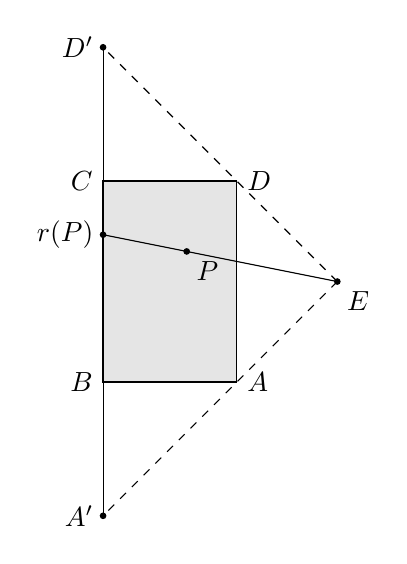
\begin{tikzpicture}[scale=0.85]
    \fill[color=white!90!black] rectangle (2,3) ;
    \draw (2,0) -- (2,3) ;
    \draw[thick]
       (2,3) node[anchor=west] {$D$} --
       (0,3) node[anchor=east] {$C$} --
       (0,0) node[anchor=east] {$B$} --
       (2,0) node[anchor=west] {$A$} ;
    \draw (0, -2) node[anchor=east] {$A'$} -- (0,0) ; \fill (0, -2) circle (0.05) ;
    \draw (0, 5) node[anchor=east] {$D'$} -- (0,3) ; \fill (0, 5) circle (0.05) ;
    \fill (3.5, 1.5) node[anchor=north west] {$E$} circle (0.05) ;
    \fill (1.25, 1.95) circle (0.05) node[anchor=north west] {$P$} ;
    \fill (0, 2.2) circle (0.05) node[anchor=east] {$r(P)$} ;
    \draw (3.5, 1.5) -- (0, 2.2) ;
    \draw[thin,dashed] (3.5, 1.5) -- (0, 5) ;
    \draw[thin,dashed] (3.5, 1.5) -- (0, -2) ;
  \end{tikzpicture}
  \caption{Extending maps from three sides to the rectangle}
  \label{fig:rectangle}
\end{figure}
%
Define $r : ABCD \to A'D'$ by mapping any point~$P$ to the intersection of $A'D'$ and the straight line through~$E$ and~$P$.
%
Now given maps $f : AB \to \RR$, $g : BC \to \RR$ and $h : CD \to \RR$ satisfying $f(B) = g(B)$ and $g(C) = h(C)$,
we may construct an extension $j : ABCD \to \RR$: transfer the maps~$f$ and~$h$ along congruences $AB \cong A'B$ and $CD \cong CD'$ to maps $f' : A'B \to \RR$ and $h' : CD' \to \RR$, let $i : A'D' \to \RR$ be an extension of $f$, $g'$ and~$h'$ obtained by an application of the previously described technique, and define $j \defeq i \circ r$.

The following lemma is an adaptation of a construction going back to~\cite{orevkov63}, see also \cite[Thm.~IV.10.1]{beeson85:_found_const_mathem}.

\begin{lemmaC}
  \label{lem:fix-point-free-map}%
  Suppose $(a_0, b_0), (a_1, b_1), (a_2, b_2), \ldots$ are open intervals with rational endpoints.
  %
  There is a continuous map $h : ([0,1] \cap \bigcup_{i \in \NN} (a_i, b_i))^2 \to [0,1]^2$ such that, $h$ has a fixed point if, and only if, there is $n \in \NN$ such that  $[0,1] \subseteq (a_0, b_0) \cup \cdots \cup (a_n, b_n)$.
\end{lemmaC}

\begin{proof}
  %
  All intervals considered in the proof have rational endpoints, so we just call them ``intervals''.
  %
  Throughout, we shall depend on decidability of the linear order on~$\QQ$, for example to test inclusion of one interval in another, or to tell whether a finite sequence of intervals with rational endpoints covers~$[0,1]$.

  We first consider the situation when the intervals $(a_i, b_i)$ are well-behaved in the following sense:
  %
  \begin{itemize}
  \item no interval shares an endpoint with $(0,1)$: $a_i, b_i \not\in \set{0,1}$ for all~$i$,
  \item there are no abutting intervals: $b_i \neq a_j$ for all $i, j$, and
  \item no interval is contained in another: $(a_i, b_i) \not\subseteq (a_j, b_j)$ for all $i \neq j$.
  \end{itemize}
  %
  Under these circumstances $(a_i, b_i)$ and $(a_j, b_j)$ are either disjoint with a positive distance between them, or they partially overlap on an open interval. Also, an interval $(a_i, b_i)$ overlaps with at most two other intervals.

  Define $V_k \defeq [0,1] \cap \bigcup_{i = 0}^k [a_i, b_i]$, and let $\partial[0,1]^2$ be the boundary of the unit square.\footnote{More precisely, $\partial[0,1]^2$ is the topological border of $[0,1]^2$ qua subset of the plane -- which need not coincide with the union of the four sides of the square.}
  %
  We construct maps
  %
  \begin{equation*}
    f_k : \partial[0,1]^2 \cup V_k^2 \to [0,1]^2
  \end{equation*}
  %
  so that each $f_k$ extends $f_{k-1}$. In addition, we ensure that if $[0,1] \neq V_k$ then~$f_k$ does not have a fixed point and its image is contained in $\partial[0,1]^2$.

  Let $f_{-1} : \partial[0,1]^2 \to \partial[0,1]^2$ be the rotation of~$\partial[0,1]^2$ by a right angle. For each $k \in \NN$, construct $f_k$ from~$f_{k-1}$ as follows:
  %
  \begin{enumerate}
  \item
    If $V_{k-1} = V_k$ then $f_k \defeq f_{k-1}$.
  \item
    %
    If $V_{k-1} \neq V_k \neq [0,1] $ then $V_k$ is~$V_{k-1}$ properly extended by $[a_k, b_k]$. The left-hand side of \cref{fig:fp-free} depicts a typical situation, where the light gray region is~$V_{k-1}$ and the dark gray the area newly contributed by~$[a_k, b_k]$.
    %
    (The assumption that the intervals are well-behaved makes sure that the dark gray strips have positive width and heights, and that at most one gap is filled at a time.)
    %
\begin{figure}[tp]
  \centering
  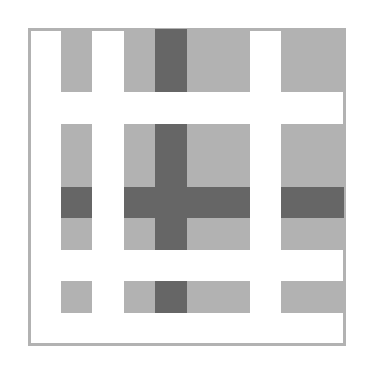
\begin{tikzpicture}[baseline=(current bounding box.center),scale=4]
    % Unit square
    \draw[very thick, color=white!70!black] (0,0) rectangle +(1,1) ;
    % Intervals: [0.1, 0.2], [0.3, 0.4], [0.5, 0.7], [0.8, 1.0]
    % column #1
    \fill[fill=white!70!black] (0.1, 0.1) rectangle +(0.1,0.1) ;
    \fill[fill=white!70!black] (0.1, 0.3) rectangle +(0.1,0.1) ;
    \fill[fill=white!70!black] (0.1, 0.5) rectangle +(0.1,0.2) ;
    \fill[fill=white!70!black] (0.1, 0.8) rectangle +(0.1,0.2) ;
    % column #2
    \fill[fill=white!70!black] (0.3, 0.1) rectangle +(0.1,0.1) ;
    \fill[fill=white!70!black] (0.3, 0.3) rectangle +(0.1,0.1) ;
    \fill[fill=white!70!black] (0.3, 0.5) rectangle +(0.1,0.2) ;
    \fill[fill=white!70!black] (0.3, 0.8) rectangle +(0.1,0.2) ;
    % column #3
    \fill[fill=white!70!black] (0.5, 0.1) rectangle +(0.2,0.1) ;
    \fill[fill=white!70!black] (0.5, 0.3) rectangle +(0.2,0.1) ;
    \fill[fill=white!70!black] (0.5, 0.5) rectangle +(0.2,0.2) ;
    \fill[fill=white!70!black] (0.5, 0.8) rectangle +(0.2,0.2) ;
    % column #4
    \fill[fill=white!70!black] (0.8, 0.1) rectangle +(0.2,0.1) ;
    \fill[fill=white!70!black] (0.8, 0.3) rectangle +(0.2,0.1) ;
    \fill[fill=white!70!black] (0.8, 0.5) rectangle +(0.2,0.2) ;
    \fill[fill=white!70!black] (0.8, 0.8) rectangle +(0.2,0.2) ;
    % new interval [0.4,0.5]
    \fill[fill=white!40!black] (0.4, 0.1) rectangle +(0.1,0.1) ;
    \fill[fill=white!40!black] (0.4, 0.3) rectangle +(0.1,0.4) ;
    \fill[fill=white!40!black] (0.4, 0.5) rectangle +(0.1,0.2) ;
    \fill[fill=white!40!black] (0.4, 0.8) rectangle +(0.1,0.2) ;
    \fill[fill=white!40!black] (0.1, 0.4) rectangle +(0.1,0.1) ;
    \fill[fill=white!40!black] (0.3, 0.4) rectangle +(0.4,0.1) ;
    \fill[fill=white!40!black] (0.5, 0.4) rectangle +(0.2,0.1) ;
    \fill[fill=white!40!black] (0.8, 0.4) rectangle +(0.2,0.1) ;
  \end{tikzpicture}
  \hfil
  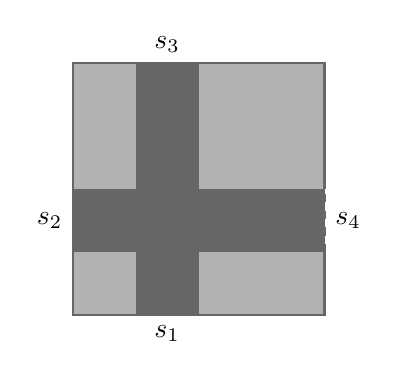
\begin{tikzpicture}[baseline=(current bounding box.center),scale=8]
    % Outer square
    \fill [fill=white!70!black] (0.3,0.3) rectangle +(0.1,0.1) ;
    \fill [fill=white!70!black] (0.3,0.5) rectangle +(0.1,0.2) ;
    \fill [fill=white!70!black] (0.5,0.5) rectangle +(0.2,0.2) ;
    \fill [fill=white!70!black] (0.5,0.3) rectangle +(0.2,0.1) ;
    \fill[fill=white!40!black] (0.4, 0.3) rectangle +(0.1,0.4) ;
    \fill[fill=white!40!black] (0.4, 0.5) rectangle +(0.1,0.2) ;
    \fill[fill=white!40!black] (0.3, 0.4) rectangle +(0.4,0.1) ;
    \fill[fill=white!40!black] (0.5, 0.4) rectangle +(0.2,0.1) ;
    \draw [thick, white!40!black, text=black]
        (0.7,0.5) -- (0.7,0.7) -- (0.5,0.7) -- (0.45,0.7) node[anchor=south] {$s_3$} -- (0.4,0.7) -- (0.3,0.7) --
        (0.3, 0.5) -- (0.3, 0.45) node[anchor=east]  {$s_2$} --
        (0.3,0.3) -- (0.45,0.3) node[anchor=north] {$s_1$} -- (0.7,0.3) -- (0.7, 0.4) ;
    \draw [very thick, white!40!black, text=black, dashed] (0.7,0.4) -- (0.7,0.45) node[anchor=west]  {$s_4$} -- (0.7,0.5) ;
  \end{tikzpicture}
  \caption{A step in the construction of~$f$ from \cref{lem:fix-point-free-map}}
  \label{fig:fp-free}
\end{figure}
    %
    We obtain~$f_k$ by extending~$f_{k-1}$ to the dark gray area separately on each rectangular component. For example, consider the central component, shown separately on the right-hand side of the figure. Because $V_k \neq [0,1]^2$ at least one of the line segments $s_1, \ldots, s_4$ is not contained in~$V_{k-1}$, say~$s_4$. Using the techniques described above, first extend $f_{k-1}$ to the other line segments, in our case $s_1, s_2, s_3$, all the while making sure that its image is contained in $\partial[0,1]^2$, and then to the entire component.
    %
    The reader may verify easily that the same approach works in other cases.
  \item
    If $V_{k-1} \neq V_k = [0,1]$ then~$[a_k, b_k]$ fills in the last gap in~$[0,1]$.
    %
    We visualize the situation by re-interpreting the right-hand side of the figure as showing~$[0,1]^2$, where
    light gray is~$V_k$ and dark gray the newly contributed area, except that this time all four segments $s_1, \ldots, s_4$ are already in the domain of~$f_{k-1}$. Pick a point in the interior of the dark gray area and declare it to be a fixed point of~$f_k$, then extend $f_k$ to the rest of the square in a piece-wise linear fashion, using the entire square as the codomain of~$f_k$.
    %
    The reader may verify that the same approach works when the dark gray area is adjacent to~$\partial[0,1]^2$, in which case it is shaped like the letter~L.
  \end{enumerate}
  %
  Notice that $V_k \neq [0,1]$ implies that~$f_k$ has no fixed points. Indeed, if $t = f_k(t)$ then $t \in \partial[0,1]^2$, which would make~$t$ a fixed point of~$f_{-1}$.

  Let $h$ be the union of $f_k$'s, restricted to $([0,1]^2 \cap \bigcup_{i \in \NN} (a_i, b_i))^2$.
  %
  We must verify that~$h$ has the required property.
  %
  If $[0,1] \subseteq (a_0, b_0) \cup \cdots \cup (a_n, b_n)$ for some $n \in \NN$, then $V_n = [0,1]$, so~$h$ has a fixed point by construction of~$f_n$.
  %
  Conversely, if~$t$ is a fixed point of~$h$ then $t \in ([0,1] \cap (a_n, b_n))^2$ for some~$n \in \NN$, hence~$f_n$ has a fixed point, which is only possible if $V_n = [0,1]$, but then $[0,1] \subseteq (a_0, b_0) \cup \cdots \cup (a_n, b_n)$ because the intervals are well-behaved.


  It remains to remove the requirement that the intervals be well-behaved.
  %
  Given any sequence of intervals $(a_0, b_0), (a_1, b_1), \ldots$, we define a new well-behaved sequence with the same union, which has a finite subcover of~$[0,1]$ if, and only if, $(a_0, b_0), (a_1, b_1), \ldots$ does.
  %
  We may then apply the above construction to the new sequence.

  Let $p_i$ be the $i$-th prime, and $P_i \defeq p_1 \cdots p_i$ the product of the first~$i$ primes.
  %
  For $i \in \NN$ and $m \in \ZZ$ let
  %
  \begin{equation*}
    \textstyle
    c_{i,m} \defeq \frac{1 + 2 m \cdot p_i}{P_i}
    \qquad\text{and}\qquad
    d_{i,m} \defeq \frac{1 + (2 m + 3) \cdot p_i}{P_{i+1}}.
  \end{equation*}
  %
  % Verification of claims:
  %
  % * the equation (1 + k · p_i)/P_i = 0 has no solutions: obvious
  % * the equation (1 + k · p_i)/P_i = 1 has no solutions: it is equivalent to 1 = p_i · (P_{i-1} - k)
  % * the equation (1 + m · p_i)/P_i = (1 + n · p_j)/P_j has no solutions:
  %   wlog assume i < j and observe that the equation is equivalent to
  %      (1 + m · p_i) P_j = (1 + n · p_j) · P_i
  %      (1 + m · p_i) p_{i+1} ⋯ p_j = 1 + n · p_j
  %      (1 + m · p_i) p_{i+1} ⋯ p_j - n · p_j = 1
  %   LHS is divisible by p_j and RHS is not.
  % From the above it follows that the intervals (c_{i,m}, d_{i,m}) have no common endpoints and the endpoints
  % are never 0 or 1.
  %
  % Verification that (c_{i,m}, d_{i,m}) are well-behaved: 
  %   c_i,m                 d_i,m         c_i,m+2                 d_i,m+2
  %   (-----------------------)            (-----------------------)
  %                     (-----------------------)
  %                    c_i,m+1                 d_i,m+1
  %
  % * c_i,m+1 < d_i,m: reduces to 2 (m + 1) < 2m + 3
  % * d_i,m < c_i,m+2: reduces to 2 m + 3 < 2 (m + 2)
  % * c_i,m+2 < d_i,m+1: reduces to 2 (m + 2) < 2 (m + 1) + 3
  %
  No two intervals $(c_{i,m}, d_{i,m})$ and $(c_{j,n}, d_{j,n})$ share an endpoint, and their endpoints are all different from $0$ and $1$. Also, for a fixed~$i$ the intervals $(c_{i,m}, d_{i,m})$ form a well-behaved cover of~$\RR$.

  We enumerate some of the intervals $(c_{i,m}, d_{i,m})$ in phases, each phase contributing finitely many intervals. In the $i$-th phase we include those $(c_{i,m}, d_{i,m})$ that are contained in $(a_0, b_0) \cup \cdots \cup (a_i, b_i)$ but are not contained in any of the intervals enumerated so far.
  %
  This way we obtain a well-behaved sequence, as the construction of $c_{i,m}$ and $d_{i,m}$ guarantees that intervals are not abutting and that their endpoints avoid $0$ and $1$; and an interval cannot contain another from the same stage, nor from an earlier one as it is too narrow.

  Obviously, the newly enumerated intervals cover at most $\bigcup_{k \in \NN} (a_k, b_k)$. They cover all of it, because any $x \in (a_k, b_k)$ is covered at the latest by the stage at which the widths of $(c_{i,m}, d_{i,m})$'s are smaller than the distance of~$x$ to the endpoints $a_k$ and $b_k$.
  %
  Finally, if $(a_0, b_0) \cup \cdots \cup (a_k, b_k)$ cover $[0,1]$, then they do so with a bit of overlap. There is a stage~$i$ such that the widths of $(c_{i,m}, d_{i,m})$'s are smaller than the overlap, so $[0,1]$ will be covered at least by the $i$-th stage.
\end{proof}

When the previous lemma is combined with Brouwer's fixed point theorem, a variant of Heine-Borel compactness of~$[0,1]$ emerges.

\begin{corollary}
  In the topos~$\TT{\mil}$, a countable cover of the closed unit interval by open intervals with rational endpoints has a finite subcover.
\end{corollary}

\begin{proof}
  Let $h : \objI^2 \to \objI^2$ be the map from \cref{lem:fix-point-free-map} for the given cover of~$\objI$.
  %
  By \cref{thm:internal-brouwer} it has a fixed point, therefore \cref{lem:fix-point-free-map} ensures that~$\objI$ is covered already by a finite subcover.
\end{proof}

We can improve on the corollary to give a variant of the Drinker paradox\footnote{The ``paradox'' states that in every non-empty pub there is a person, such that if the person is drinking then everyone is drinking. It is a non-constructive principle~\cite{warren2018drinker}.} for sufficiently tame predicates on the closed unit interval.

\begin{proposition}[Drinking Buddies Principle]
  \label{prop:drinking-buddies}%
  In the topos~$\TT{\mil}$, suppose $U$ is a countable union of open intervals with rational endpoints.
  There are $x, y \in \objI$ such that $x \in U \land y \in U$ if, and only if, $\all{z \in \objI} z \in U$.
\end{proposition}

\begin{proof}
  Let $(a_0, b_0), (a_1, b_1), \ldots$ be a sequence of intervals with rational endpoints and $U \defeq \bigcup_{i \in \NN} (a_i, b_i)$ and $h : (\objI \cap U)^2 \to \objI^2$ the map from \cref{lem:fix-point-free-map} for the given intervals. We claim that $U$ is a $\neg\neg$-stable subset of~$\RR$. One way to see this is to recall from \cref{lem:lt-stable} that~$<$ is $\neg\neg$-stable, and observe that there is a map $t : \RR \to \RR$ such that $U = \set{x \in \RR \such t(x) > 0}$, for instance a weighted sum of “tent maps” errected on the intervals,
  %
  \begin{equation*}
    \textstyle
    t(x) = \sum_{n \in \NN} 2^{-n} \cdot \max (0, 1 - |\max (a_n, \min (b_n, x)) - (a_n + b_n)/2|).
  \end{equation*}
  %
  Therefore, \cref{thm:partial-brouwer} applies to~$h$ to give $(x, y) \in \objI^2$ such that if $x, y \in U$ then $h(x,y) = (x,y)$, whence $\objI \subseteq U$ by \cref{lem:fix-point-free-map}.
\end{proof}

We are not certain what the principle is good for, apart from obliging one to test its veracity with a buddy in a pub.

%%% Local Variables:
%%% mode: latex
%%% TeX-master: "countable-reals"
%%% End:
